\section{Zweidimensionales Punktdiagramm}

Da das zweidimensionale Punktdiagramm weit verbreitet ist, sind sich Betrachter an diese Darstellung gewöhnt. Oft werden die Punkte in Diagramm durch eine Linie verbunden, was den Verlauf der abgebildeten Datenwerte verdeutlicht, besonders in Medien, zum Beispiel für die Darstellung von Börsenkursen. 

Aus diesem Grund wurde als erstes Beispiel das zweidimensionale Punktdiagramm (beziehungsweise das Liniendiagramm, falls Linien hinzugefügt werden) ausgewählt.


\subsection{Applikation}

\begin{figure}[!htbp]
	\centering
	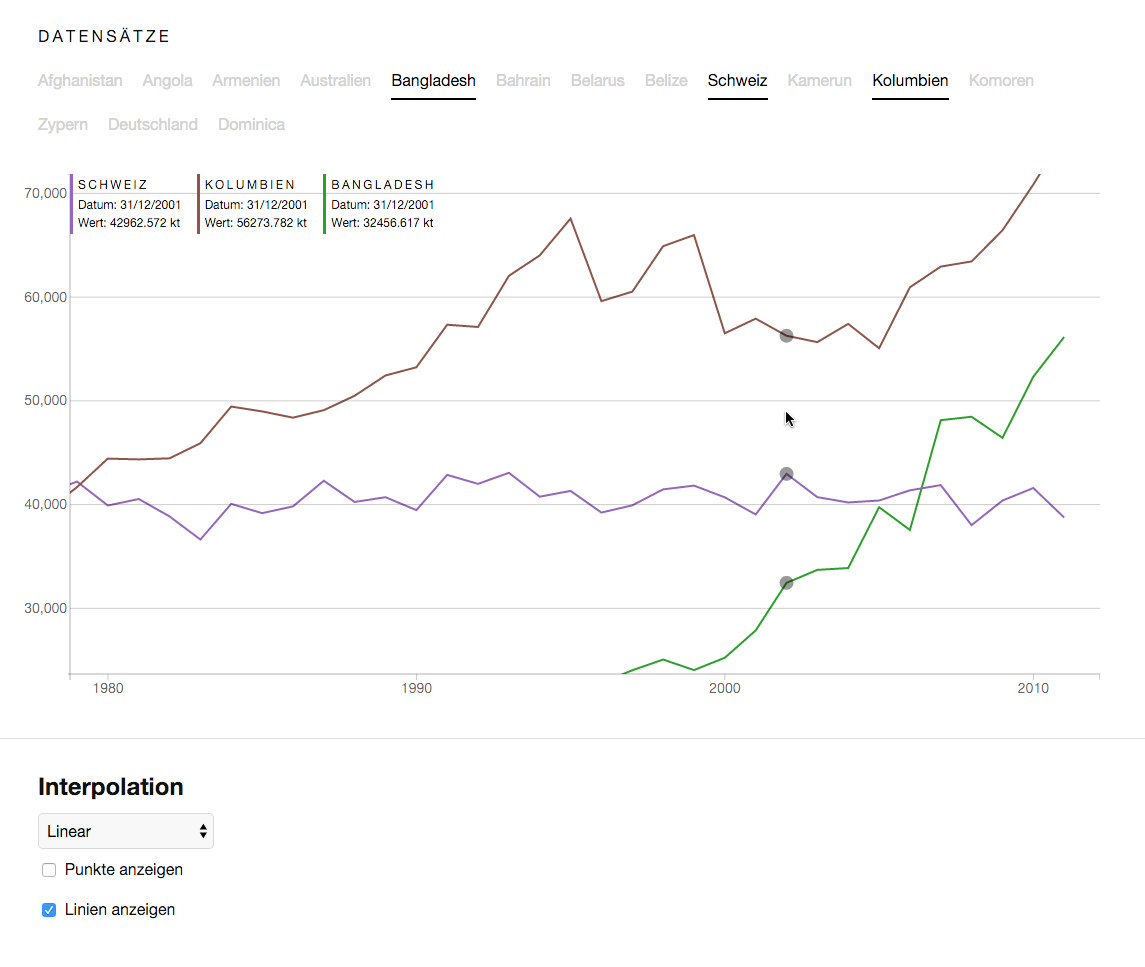
\includegraphics[width=\linewidth]{images/2dline}
	\caption{Screenshot der Oberfläche der Applikation (zweidimensionales Liniendiagramm / Punktdiagramm)}
	\label{fig:screenshot}
\end{figure}

Der Screenshot in Abbildung \ref{fig:screenshot} zeigt die entwickelte Applikation. Es sind Datensätze \cite{worldbank} zum $CO_2$-Verbrauch von 15 Ländern vorhanden, drei davon sind im Diagramm eingeblendet. Der Name des Tests in der Applikation lautet \texttt{layout}.

\textbf{Achsen.} Es wurden Achsen mit linearer Skala für die Applikation gewählt. Beschriftungen und Markierungen, sogenannte \textit{Ticks}, sind vorhanden. Die Ticks auf der Ordinatenachse (y-Achse) wurden in Richtung der Innenseite des Diagramms verlängert, so dass ein Gitter entsteht.

Falls in einem Diagramm mehrere Datensätze gleichzeitig dargestellt werden sollen, wie es der Fall in Abbildung \ref{fig:screenshot} ist, so müssen die abgebildeten Werte die gleiche Einheit (zum Beispiel Meter, Kilogramm, Franken) besitzen. Bei der gleichzeitigen Darstellung von mehreren Datensätzen mit verschiedenen Einheiten in einem Diagramm muss für jede vorhandene Einheit eine eigene Achse und Skala gezeichnet werden.

\textbf{Datenpunkte.} Die Applikation bietet an, die Daten als Punkte und bzw. oder verbunden durch eine Linie anzuzeigen. In Abbildung \ref{fig:screenshot} unten wird durch Kontrollkästchen ermöglicht, die Anzeige zu verändern.

\textbf{Layout und Textformatierung.} Für den Schritt \textit{Übersicht} ist das Layout und auch die Formatierung des Textes von Bedeutung. Eine klare Oberflächenstruktur nach modernen Minimalismus (nach Designtrends wie \textit{Flat Design} oder \textit{Material Design}) wurde geschaffen, bei denen der Inhalt im Vordergrund steht. "`Benutzer betrachten keine Details, sie benutzen Details."' \cite{minimalism}.

Zur besseren Orientierung des Benutzers wird hier das Prinzip von "`\textit{pop}"' und "`\textit{unpop}"' von Text, das von Erik Kennedy \cite{pop} beschrieben wurde, berücksichtigt: Durch die Anpassung der Typographie kann ein Text hervorgehoben beziehungsweise in den Hintergrund gestellt werden. Folgende Eigenschaften von Texten im Diagramm werden in der Applikation entsprechend der Wichtigkeit angepasst:

\begin{itemize}
	\item Grösse (grösser bzw. kleiner)
	\item Farbe (grösserer bzw. kleinerer Kontrast)
	\item Schriftstärke (fetter bzw. leichter)
	\item Schriftart (Grossschreibung bzw. Kleinschreibung)
	\item Laufweite (kleiner bzw. grösser)
	\item Unterstreichung (unterstrichen bzw. nicht unterstrichen)
\end{itemize}

\textbf{Linien.} Der Verlauf der abgebildeten Datenwerte wird verdeutlicht, indem die Punkte im Diagramm durch eine Linie verbunden werden. Die lineare Interpolation wurde durch ein selbstgeschriebenes Modul implementiert. Weitere Interpolationen, wie der \textit{Kubisch Hermitescher Spline} oder \textit{Basis-Spline}, wurden mit D3 implementiert und können auf das Diagramm angewendet werden.

\begin{figure}[!htbp]
	\begin{minipage}{\textwidth}
		\centering
		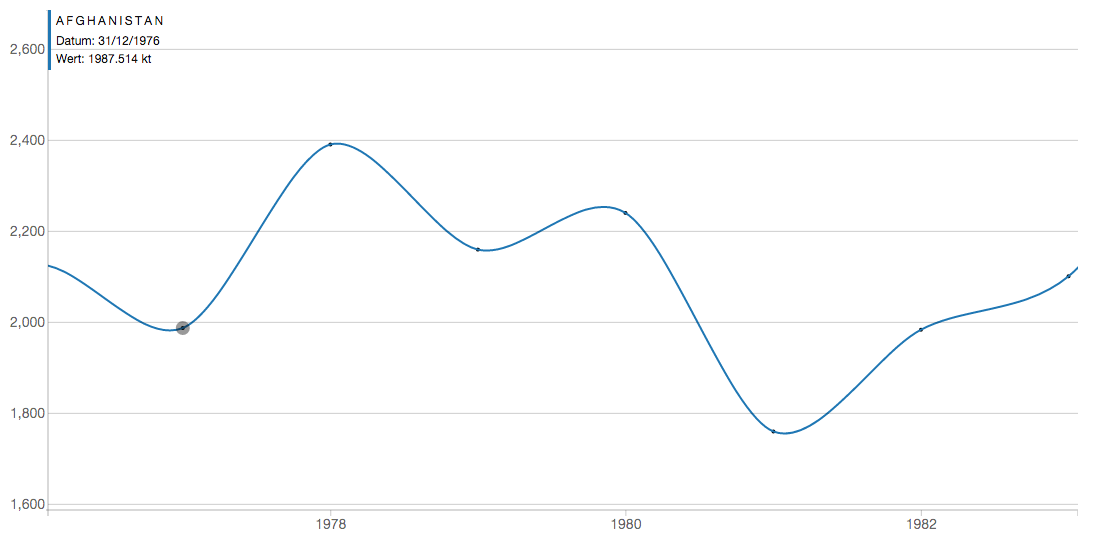
\includegraphics[width=\linewidth]{images/cardinal}
	\end{minipage}
	\begin{minipage}{\textwidth}
		\centering
		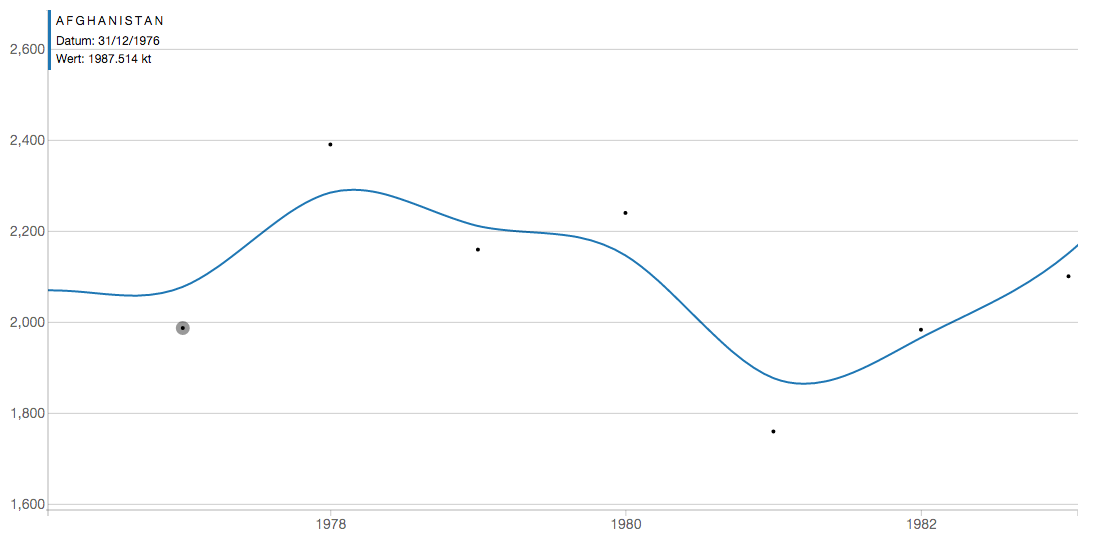
\includegraphics[width=\linewidth]{images/basis}
	\end{minipage}
	\caption[Beispiele von Interpolationen und Zoom]{1. Beispiele von Interpolationen im Diagramm. V.o.n.u: Kubisch Hermitescher Spline, Basis-Spline. 2. Gezoomte Ansicht}
	\label{fig:vergleich}
\end{figure}

Verschiedene Farben von Linien ermöglichen die Zuordnung von Datensätzen. Die den Datensätzen zugewiesenen Farben werden in der Detailanzeige dargestellt.

\textbf{Zoom.} Der Schritt \textit{Zoomen} wurde im Diagramm umgesetzt. Es kann durch Scrollen gezoomt werden, indem die Skalierungen der Achsen verändert werden. Die Programmlogik wurde mittels D3 implementiert. 

Es gibt zahlreiche interaktive Diagramme, in denen nur der Zoom durch Veränderung der Skalierung der Abszisse möglich ist. Dabei wird nach jedem Zoom-Vorgang die Skalierung der Ordinate and die Daten neu angepasst oder überhaupt nicht verändert.

Diese Zoom-Strategie verwirrt den Benutzer, weil sich die Skalierungen der Achsen nicht gleichmässig beim Zoom verändern: Er nimmt ein Dehnen bzw. Zusammendrücken des Diagramms wahr. Der Benutzer ist es sich gewöhnt, dass die beiden Skalierungen stets im gleichen Verhältnis stehen; dies ist auch beim Zoom bei Smartphones üblicherweise der Fall. Deshalb wurde diese Zoomstrategie bevorzugt und umgesetzt.

\textbf{Datensatzauswahl.} In diesem Beispiel (Abbildung \ref{fig:screenshot}) können Linien ein- und ausgeblendet werden, die Datensätzen für 15 Länder entsprechen. Dieser Vorgang gehört zum Schritt \textit{Filtern}. Aktivierte, angezeigte Datensätze werden nach den Prinzipien von Kennedy hervorgehoben, nicht aktivierte, versteckte Datensätze sind in den Hintergrund gestellt.

\textbf{Tooltip und Detailanzeige.} Beim Tooltip wird der der Maus am nächsten liegende Datenpunkt jedes Datensatzes markiert und erscheint in der Detailanzeige. In der Detailanzeige werden, falls im Datensatz vorhanden, weitere Informationen (Datenspalten) und genaue x- und y-Werte mit Einheit angezeigt. Dieser Vorgang entspricht dem Schritt \textit{Details auf Abruf}.

\textbf{Dynamik der Applikation.} Der Screenshot dieses Beispiels (Abbildung \ref{fig:screenshot}) ist das Resultat der Anzeige der Applikation, die für einen bestimmten Datensatz konfiguriert ist. Elemente des Diagramms, wie der Wertebereich der Achsen, die Datensatzauswahl, Tooltip und Detailanzeige, werden dynamisch generiert, so dass diese Module ohne weitere Einstellung auch für andere Datensätze funktionieren.

